The system employs a hybrid recommendation strategy that adapts to the user's interaction history, integrating graph-based methods (akin to a Graph-\ac{rag} approach) with an expert model to provide relevant and diverse suggestions. This methodology addresses the complex nature of \textbf{RQ2} by combining contextual, collaborative, and deep learning-based signals. The overall procedure, illustrated in Figure~\ref{FIG:HYBRID_RECS}, begins by assessing the user's interaction history with the \texttt{FalkorDBRecommender} module, which is responsible for graph-based recommendations and explanations.

\begin{figure}[Hybrid Recommendations Diagram]{FIG:HYBRID_RECS}{A diagram of the generation of hybrid recommendations.}
    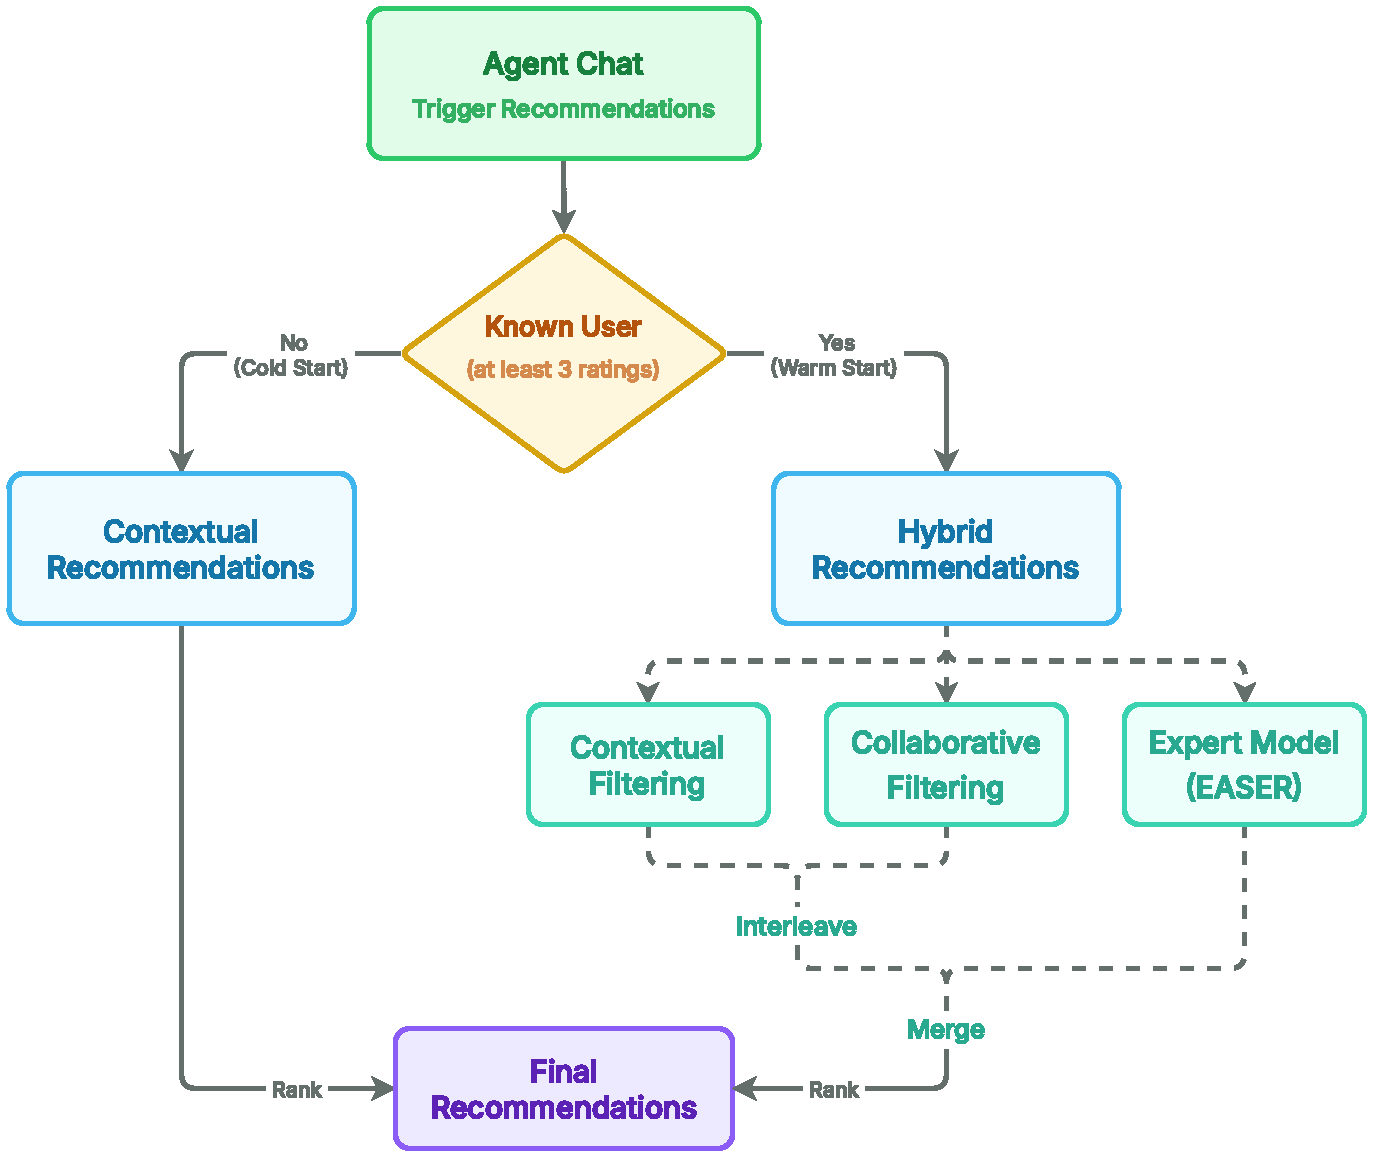
\includegraphics[width=\textwidth]{recommendations_hybrid.pdf}
\end{figure}

A key decision point in the workflow is whether the user has rated at least three items. If not, the system operates in a ``cold-start'' mode, relying exclusively on a contextual recommendation method.

\paragraph{Contextual Recommendations for Cold-Start Scenarios}
In cold-start situations or when a user's request is highly specific, the system utilizes a graph-based contextual recommender. This component provides the system with its contextual reasoning capabilities, akin to a Graph-\ac{rag} approach. The process for generating these recommendations is depicted in Figure~\ref{FIG:REC_CTX}.

\begin{figure}[Contextual Recommendations Diagram]{FIG:REC_CTX}{A diagram of the contextual recommendation process.}
    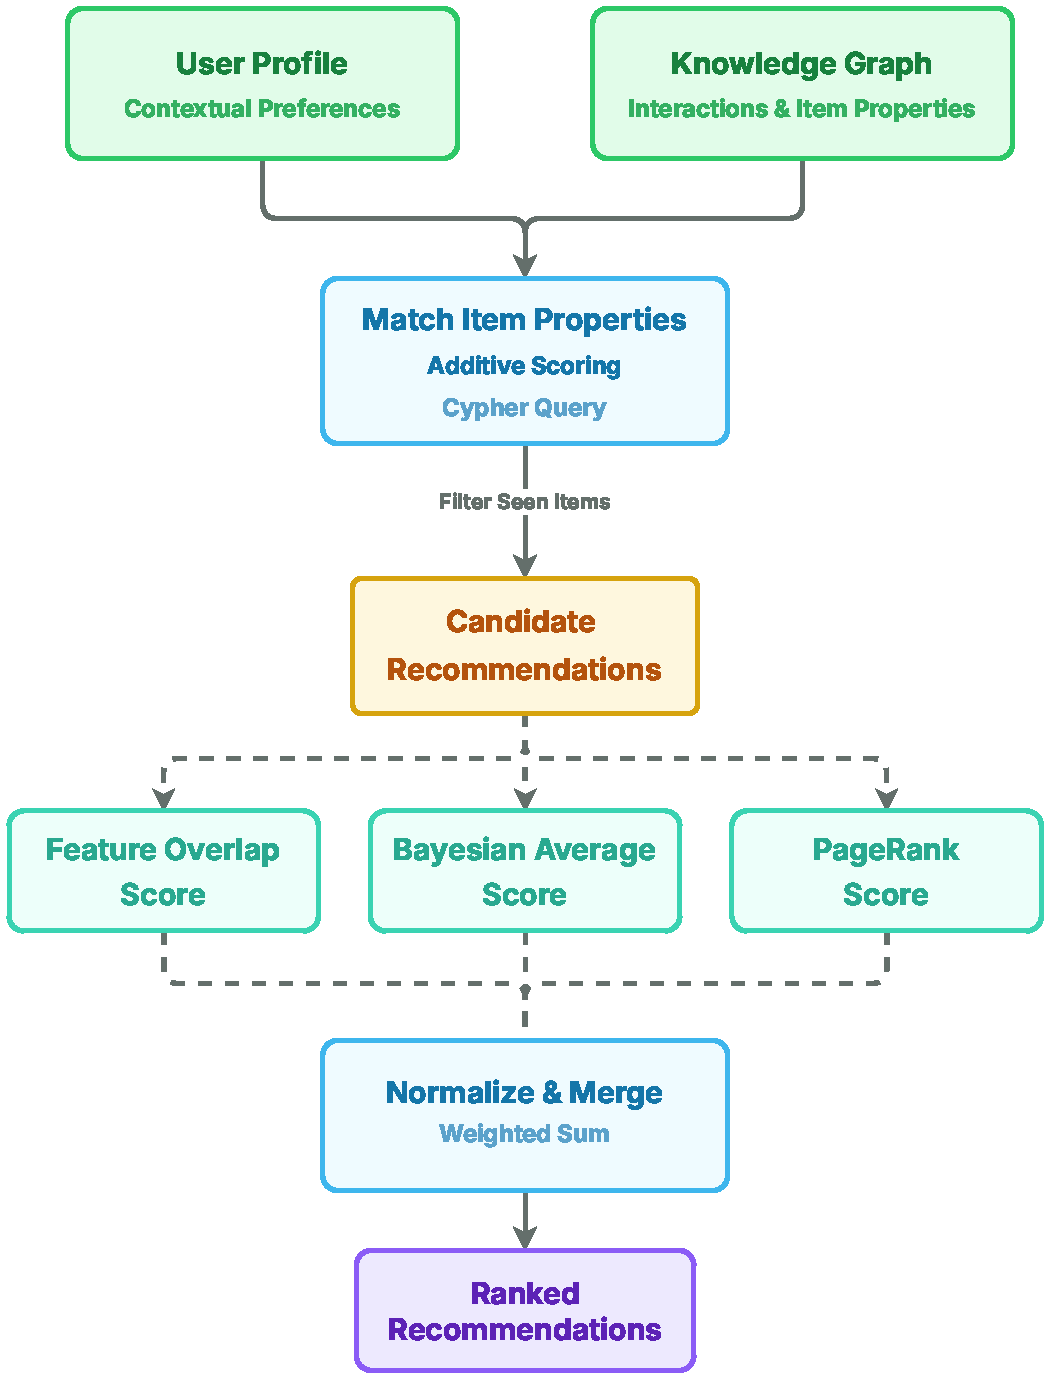
\includegraphics[width=0.8\textwidth]{recommendations_contextual.pdf}
\end{figure}

The process begins by translating the user's active contextual preferences into a Cypher query to retrieve items with matching properties from the \ac{kg}. A representative example of this query is provided in Appendix~\ref{AP:CYPHER_QUERIES}, Code~\ref{COD:QUERY_1}. After filtering out items previously seen by the user, each candidate item is evaluated using a weighted combination of three distinct signals:
\begin{compactitem}[\textbullet]
    \item \textbf{Feature Overlap Score:} A score based on how well an item's attributes match the user's stated contextual preferences.
    \item \textbf{Bayesian Average Score:} To ensure that the popularity score is reliable and not skewed by items with very few ratings, a Bayesian Average is used. This formula, shown in Equation~\ref{EQ:BAYESIAN_AVERAGE}, smooths the average rating of an item by incorporating the global average rating across all items.
    
    \vspace{5pt}
    \begin{equation}[EQ:BAYESIAN_AVERAGE]{Bayesian Average}
        \text{BayesianAverage} = \frac{v}{v+m} \cdot R + \frac{m}{v+m} \cdot C
    \end{equation}
    \noindent where $v$ is the number of ratings for the item, $R$ is the item's own average rating, $m$ is a minimum number of ratings required for confidence, and $C$ is the global average rating across all items.

    \item \textbf{PageRank Score:} To measure the structural importance of an item within the user-item interaction graph, the PageRank algorithm \cite{PAGERANK} is precomputed for all items, as described in Equation~\ref{EQ:PAGERANK}.

    \vspace{5pt}
    \begin{equation}[EQ:PAGERANK]{PageRank}
        PR_{i}={\frac  {1-d}{n}}+d\,\sum _{{j\in \{1,\dots ,n\}}}{\frac  {PR_{j}}{c_{j}}}
    \end{equation}
    \noindent where $PR_i$ is the PageRank score of item $i$, $n$ is the total number of items, $d$ is a damping factor (typically 0.85), and the sum is over all items $j$ that have a rating for item $i$, with $c_j$ being the total number of outgoing ratings from item $j$. The final ranked list of items represents a context-aware set of recommendations that can immediately respond to the user's needs.
\end{compactitem}

\paragraph{Hybrid Recommendations for Existing Users}
For users with an established history of at least three rated items, the system enhances its recommendations by incorporating \acl{cf} and an expert model. In this mode, the final list of recommendations is a blend of results from three sources: the contextual method described previously, a \acl{cf} method, and the \texttt{EASER} model.

The \acl{cf} component, illustrated in Figure~\ref{FIG:RECS_CF}, identifies users with similar tastes to the target user through Cypher queries. It achieves this by finding ``neighbors'' in the \ac{kg} who have positively rated the same items as the target user. The items liked by these neighbors, which the target user has not yet seen, are then considered as potential recommendations and ranked by their Bayesian average score. A representative example of these queries is included in Appendix~\ref{AP:CYPHER_QUERIES}, Code~\ref{COD:QUERY_2}.

\begin{figure}[Collaborative Filtering Recommendations Diagram]{FIG:RECS_CF}{A diagram of the \acl{cf} recommendation process.}
    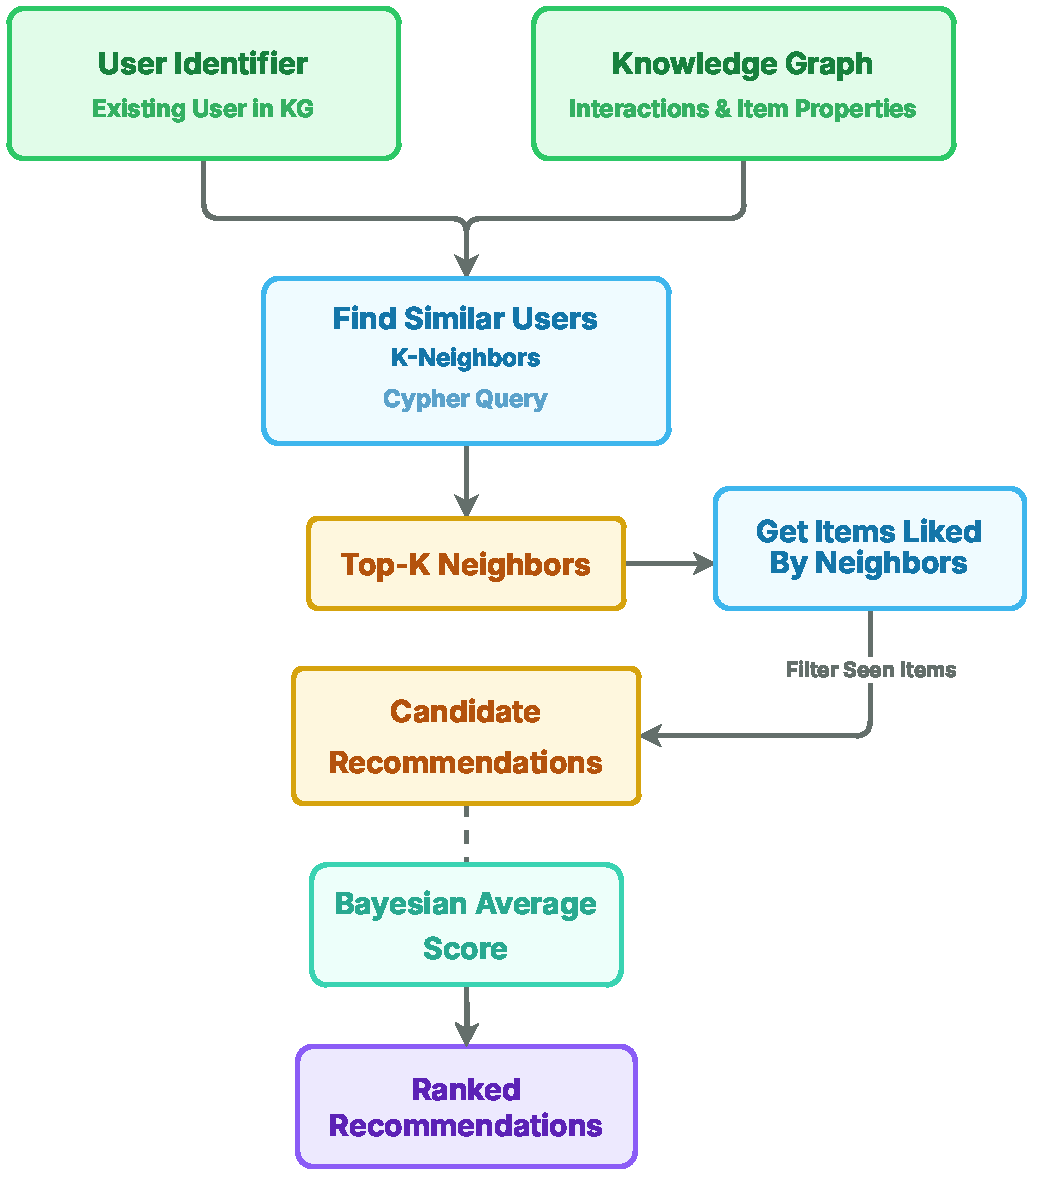
\includegraphics[width=0.8\textwidth]{recommendations_cf.pdf}
\end{figure}

Finally, recommendations from the contextual and \acl{cf} methods are combined with a list of high-quality recommendations from the \texttt{EASER} model. The final set of recommendations is generated by interleaving the ranked lists from all three sources, ensuring a diverse yet personalized output.
